% ================================================================= DEMO VÀ ĐÈN TIN CẬY
\section{Bản demo và đèn tin cậy}
\label{sec:demo}

Nhóm đã xây bản demo chạy được, tách thành hai tầng: \texttt{demo/core.py} chứa toàn bộ logic, không phụ
thuộc thư viện giao diện và có bộ kiểm thử riêng; \texttt{demo/app.py} là giao diện web một trang bằng
Gradio, chạy trên máy cá nhân bằng lệnh \texttt{python demo/app.py}.

\subsection{Bố cục}

Màn hình gồm bốn khối, xếp theo thứ tự người xem cần biết:

\begin{enumerate}[leftmargin=1.6em,itemsep=3pt]
\item \textbf{Đầu vào}: tải tệp EDF/WFDB/CSV hoặc chọn bản ghi mẫu; chọn kênh tự động (quy tắc PSD mù
nhãn) hoặc thủ công. Nếu chọn bản ghi ADFECGDB thì hệ thống \textit{tự động} dùng checkpoint chưa từng
thấy bản ghi đó, để kết quả hiển thị là kết quả trung thực.
\item \textbf{Tín hiệu qua từng bước}, năm tab: thô, đã lọc kèm vạch nhịp mẹ, sau khử mẹ kèm vạch nhịp
thai thật nếu có nhãn, xác suất từng mẫu kèm ngưỡng, và kết quả. Người xem kéo thả phóng to được.
\item \textbf{Nhịp tim thai theo thời gian}, tô vùng bình thường 110--160 nhịp/phút.
\item \textbf{Bốn thẻ số}: nhịp tim trung bình, số nhịp, \textbf{đèn tin cậy}, thời gian xử lý. Nếu có
nhãn thì hiện thêm Se/PPV/F1/jitter.
\end{enumerate}

Chân trang cố định: \textit{``Bản mẫu nghiên cứu. Không phải thiết bị y tế. Không dùng cho chẩn đoán.''}

\begin{figure}[H]\centering
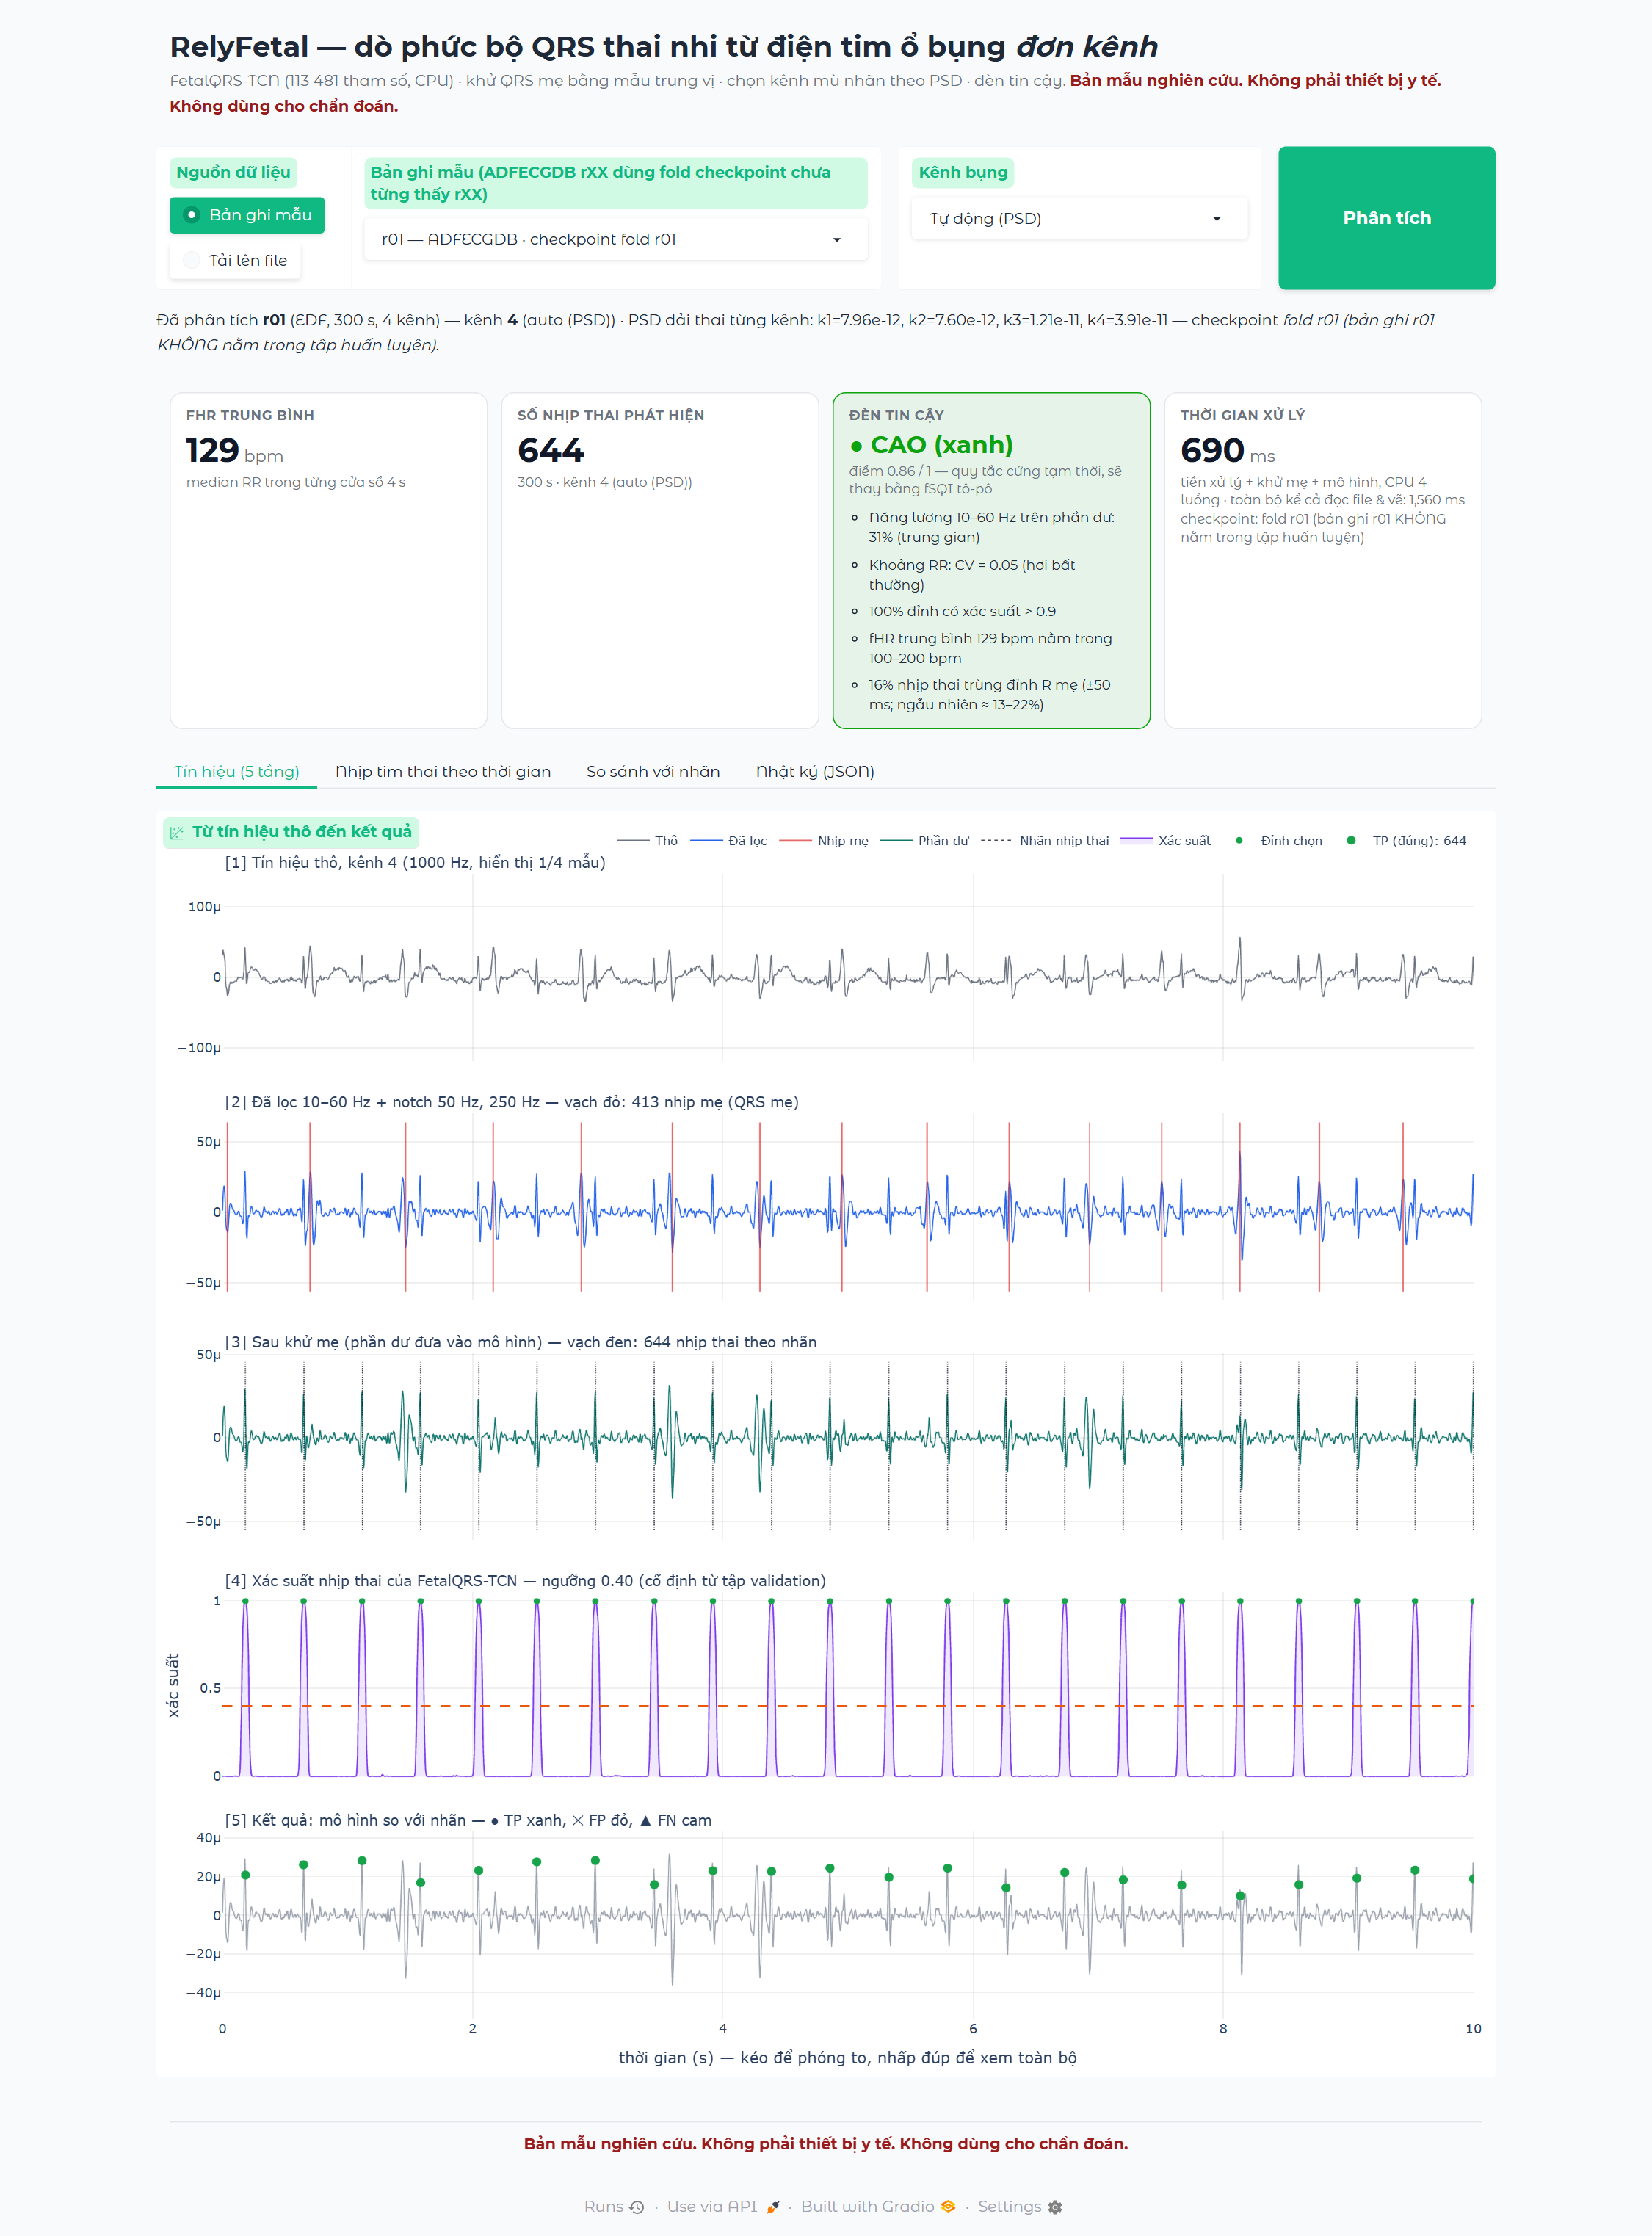
\includegraphics[width=0.92\textwidth]{figs/fig11_demo_r01.png}
\caption{Ảnh chụp giao diện thật trên r01, kênh chọn tự động, checkpoint chưa thấy r01. Năm tầng tín
hiệu, 644 nhịp, đèn xanh, 690\,ms xử lý cho 5 phút tín hiệu.}
\label{fig:demo_r01}
\end{figure}

\begin{figure}[H]\centering
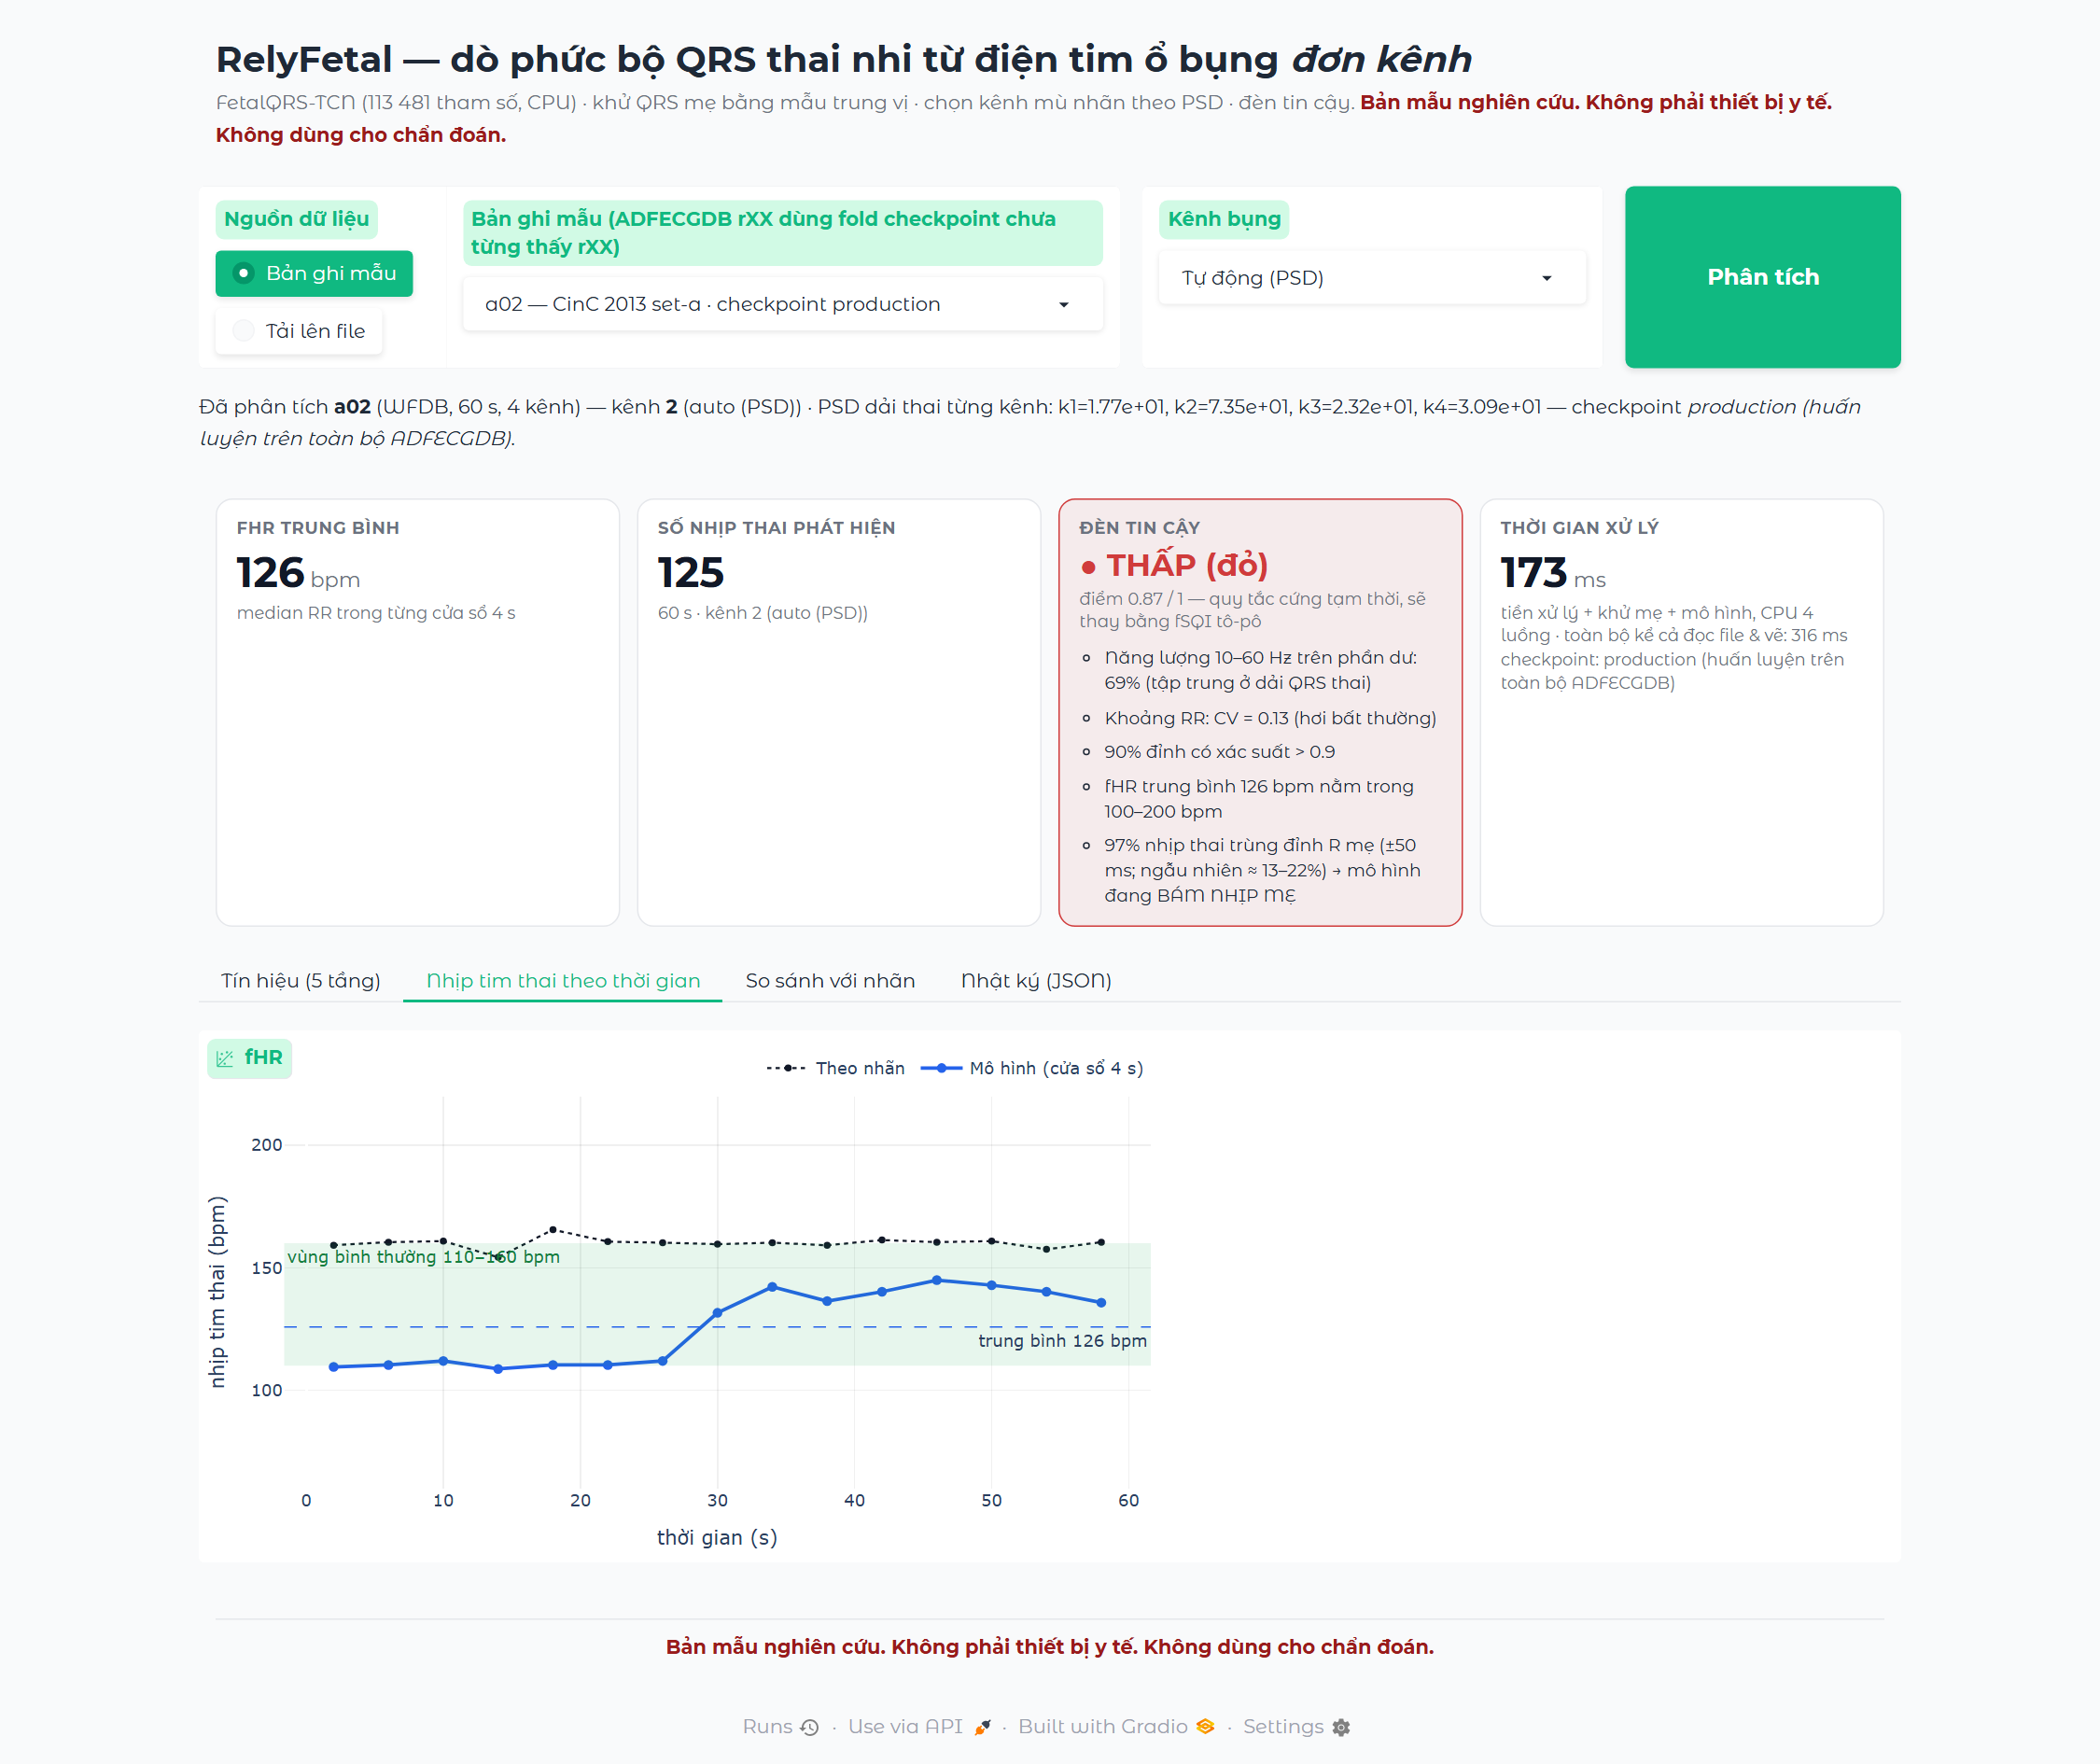
\includegraphics[width=0.92\textwidth]{figs/fig12_demo_a02.png}
\caption{Ảnh chụp trên a02, bản ghi tệ nhất của CinC 2013, zero-shot. Đèn \textbf{đỏ} vì 97\% nhịp
``thai'' trùng đỉnh R mẹ. Đồ thị nhịp tim cho thấy đúng cơ chế thất bại: đường mô hình bám ở nhịp mẹ
($\approx$126) trong khi nhãn ở $\approx$160 nhịp/phút. Hệ thống tự phát hiện và từ chối, thay vì báo
sai.}
\label{fig:demo_a02}
\end{figure}

\subsection{Đèn tin cậy}

Đây là thành phần biến demo từ ``một bộ dò QRS nữa'' thành thứ khác biệt. Phiên bản hiện tại dùng
\textbf{luật cứng} kết hợp bốn dấu hiệu, mỗi dấu hiệu chỉ dùng chính tín hiệu và đầu ra mô hình, không
dùng nhãn:

\begin{table}[H]\centering\small
\caption{Bốn dấu hiệu của đèn tin cậy phiên bản luật cứng. Trọng số cộng lại thành điểm 0--1; xanh nếu
$\geq 0{,}75$, vàng nếu $\geq 0{,}45$, đỏ nếu thấp hơn. Có một luật ghi đè: nếu hơn 60\% nhịp ``thai''
trùng đỉnh R mẹ thì đèn đỏ bất kể điểm, vì đó là dấu hiệu bộ dò đang bám nhầm vào tim mẹ.}
\label{tab:dentincay}
\begin{tabular}{@{}L{4.6cm} L{6.6cm} C{1.6cm}@{}}
\toprule
\textbf{Dấu hiệu} & \textbf{Ý nghĩa} & \textbf{Trọng số} \\
\midrule
Tỉ lệ năng lượng 10--60\,Hz trên phần dư & Phần dư còn chứa QRS thai hay chỉ còn nhiễu & 0,2 \\
Hệ số biến thiên khoảng RR & Nhịp đều là dấu hiệu bắt đúng; nhịp loạn là dấu hiệu bắt nhiễu & 0,3 \\
Tỉ lệ đỉnh có xác suất $> 0{,}9$ & Mô hình có tự tin vào các đỉnh nó chọn không & 0,3 \\
Nhịp tim nằm trong 100--200 nhịp/phút & Kiểm tra sinh lý & 0,2 \\
\bottomrule
\end{tabular}
\end{table}

Luật này được cố định trước khi chạy, rồi chấm trên 15 bản ghi có nhãn.

\begin{table}[H]\centering\small
\caption{Đèn tin cậy chấm trên 15 bản ghi có nhãn, kênh chọn tự động. ADFECGDB dùng checkpoint chưa
thấy bản ghi; CinC 2013 dùng checkpoint production, zero-shot.}
\label{tab:den15}
\begin{tabular}{@{}L{1.4cm} L{2.0cm} C{1.0cm} C{1.6cm} C{2.0cm} C{1.4cm} C{2.0cm}@{}}
\toprule
\textbf{Bản ghi} & \textbf{Bộ} & \textbf{Kênh} & \textbf{F1 thật} & \textbf{Đèn} & \textbf{Điểm} &
\textbf{Độ trễ} \\
\midrule
r01 & ADFECGDB & 4 & 100,00 & \tot{xanh} & 0,86 & 758\,ms \\
r04 & ADFECGDB & 2 & 99,76 & vàng & 0,74 & 778\,ms \\
r07 & ADFECGDB & 2 & 100,00 & \tot{xanh} & 0,80 & 661\,ms \\
r08 & ADFECGDB & 4 & 99,77 & \tot{xanh} & 0,90 & 720\,ms \\
r10 & ADFECGDB & 1 & 96,54 & \tot{xanh} & 0,92 & 732\,ms \\
\midrule
a03 & CinC 2013 & 1 & 100,00 & \tot{xanh} & 0,99 & 124\,ms \\
a04 & CinC 2013 & 4 & 100,00 & \tot{xanh} & 0,94 & 131\,ms \\
a05 & CinC 2013 & 4 & 100,00 & \tot{xanh} & 0,94 & 137\,ms \\
a08 & CinC 2013 & 4 & 100,00 & \tot{xanh} & 1,00 & 144\,ms \\
a01 & CinC 2013 & 2 & 59,18 & vàng & 0,57 & 118\,ms \\
a06 & CinC 2013 & 1 & 42,75 & vàng & 0,48 & 119\,ms \\
a07 & CinC 2013 & 2 & 29,82 & vàng & 0,48 & 125\,ms \\
a10 & CinC 2013 & 2 & 21,05 & vàng & 0,63 & 127\,ms \\
a02 & CinC 2013 & 2 & 21,75 & \xau{đỏ} & 0,87$^{*}$ & 132\,ms \\
a09 & CinC 2013 & 2 & 16,96 & \xau{đỏ} & 0,27 & 127\,ms \\
\bottomrule
\multicolumn{7}{@{}l}{\scriptsize $^{*}$ điểm cao nhưng bị luật ghi đè: 89\% nhịp ``thai'' trùng đỉnh R
mẹ --- bộ dò bám nhầm vào tim mẹ.}
\end{tabular}
\end{table}

\begin{table}[H]\centering\small
\caption{Tổng hợp theo màu đèn.}
\label{tab:den_tonghop}
\begin{tabular}{@{}C{2.0cm} C{2.2cm} C{2.6cm} C{2.6cm} C{2.6cm}@{}}
\toprule
\textbf{Đèn} & \textbf{Số bản ghi} & \textbf{F1 trung bình} & \textbf{F1 thấp nhất} & \textbf{F1 cao nhất} \\
\midrule
\tot{Xanh} & 8 & \textbf{99,54} & 96,54 & 100,00 \\
Vàng & 5 & 50,51 & 21,05 & 99,76 \\
\xau{Đỏ} & 2 & 19,36 & 16,96 & 21,75 \\
\bottomrule
\end{tabular}
\end{table}

\begin{ghichu}[title={Điều quan trọng nhất trong bảng \ref{tab:den_tonghop}}]
\textbf{Không có bản ghi nào bị đèn xanh mà F1 dưới 96.} Tức là luật cứng đơn giản này, dù chưa dùng
đặc trưng topo, đã đạt tính chất cần thiết nhất của một cổng an toàn: \textit{khi nó nói ``tin được'' thì
tin được}. Sai số duy nhất là theo chiều thận trọng --- r04 bị đèn vàng dù F1 là 99,76.

Trên CinC 2013, nếu chỉ trả lời khi đèn xanh thì macro F1 của phần được trả lời là \textbf{100,00}
trên 4/10 bản ghi, và hệ thống \textit{từ chối} 6 bản ghi còn lại thay vì báo sai. Đây là minh hoạ cụ thể
cho đóng góp C3 trước khi thay luật cứng bằng chỉ số topo học được.
\end{ghichu}

\subsection{Kịch bản trình bày ba phút}

\begin{table}[H]\centering\small
\caption{Kịch bản demo. Phút cuối là phần quan trọng nhất.}
\label{tab:kichban}
\begin{tabular}{@{}C{1.6cm} L{5.2cm} L{7.4cm}@{}}
\toprule
\textbf{Thời điểm} & \textbf{Thao tác} & \textbf{Điều cần nói} \\
\midrule
0:00--0:30 & Nạp r01, bấm Phân tích & Năm phút tín hiệu, xử lý xong dưới một giây \\
0:30--1:30 & Lướt năm tab tín hiệu & Đây là chỗ nhịp thai bị chôn; đây là sau khi trừ mẹ \\
1:30--2:00 & Bật so sánh với nhãn & 644 nhịp, không sót, không thừa, F1 100 \\
2:00--3:00 & \textbf{Nạp a02, bản ghi tệ nhất} & Đèn chuyển đỏ. Hệ thống tự biết nó bám nhầm tim mẹ và
từ chối trả lời, thay vì báo một con số sai \\
\bottomrule
\end{tabular}
\end{table}

Demo chỉ chạy trên ca đẹp thì ai cũng làm được. Demo dám chạy trên ca xấu và \textit{tự thừa nhận} mới
là điểm khác biệt.
